\documentclass[zavrsnirad]{fer}
% Dodaj opciju upload za generiranje konačne verzije koja se učitava na FERWeb
% Add the option upload to generate the final version which is uploaded to FERWeb

\usepackage{blindtext}
\usepackage{listings}
\usepackage{hyperref}
\usepackage{placeins}
\definecolor{darkgreen}{rgb}{0, 0.6, 0}

\lstdefinelanguage{CSharp}{
	language=[Sharp]C,
	morekeywords={
		abstract, as, base, bool, break, byte, case, catch, char, checked, class, const, continue,
		decimal, default, delegate, do, double, else, enum, event, explicit, extern, false, finally,
		fixed, float, for, foreach, goto, if, implicit, in, int, interface, internal, is, lock, long,
		namespace, new, null, object, operator, out, override, params, private, protected, public,
		readonly, ref, return, sbyte, sealed, short, sizeof, stackalloc, static, string, struct, switch,
		this, throw, true, try, typeof, uint, ulong, unchecked, unsafe, ushort, using, virtual, void,
		volatile, while, async, await, var, dynamic
	},
	sensitive=true,
	morecomment=[l]{//},
	morecomment=[s]{/*}{*/},
	morestring=[b]",
}

\lstdefinelanguage{GraphQL}{
	keywords={
		query, mutation, subscription, type, input, interface, union, scalar, enum, fragment, on,
		implements, extend, schema, directive, extends, null, true, false
	},
	keywordstyle=\color{blue}\bfseries,
	ndkeywords={
		__schema, __type, __typename, __directive, __inputValue, __field, __enumValue, __typeKind
	},
	ndkeywordstyle=\color{violet}\bfseries,
	sensitive=true,
	morecomment=[s]{""" }{ """},
	morecomment=[s]{"""}{"""},
	morestring=[b]{"},
	morestring=[s]{"""}{"""}
}

\lstdefinelanguage{Javascript}{
	keywords={typeof, new, true, false, catch, function, return, null, catch, switch, var, if, in, while, do, else, case, break},
	keywordstyle=\color{blue}\bfseries,
	ndkeywords={class, export, boolean, throw, implements, import, this, static, async},
	ndkeywordstyle=\color{purple}\bfseries,
	identifierstyle=\color{black},
	sensitive=false,
	comment=[l]{//},
	morecomment=[s]{/*}{*/},
	commentstyle=\color{purple}\ttfamily,
	stringstyle=\color{red}\ttfamily,
	morestring=[b]',
	morestring=[b]"
}

\lstset{
	basicstyle=\linespread{0.8}\ttfamily,
	keywordstyle=\color{blue}\bfseries,
	commentstyle=\color{darkgreen}\itshape,
	stringstyle=\color{red},
	showstringspaces=false,
	numberstyle=\tiny\color{gray},
	numbersep=5pt,
	tabsize=2,
	breaklines=true,
	showtabs=false,
	showspaces=false,
	showlines=true,
	frame=single,
	backgroundcolor=\color{white}
}

%--- PODACI O RADU / THESIS INFORMATION ----------------------------------------

% Naslov na engleskom jeziku / Title in English
\title{GraphQL-based server monitoring system}

% Naslov na hrvatskom jeziku / Title in Croatian
\naslov{Sustav za praćenje stanja poslužitelja temeljen na jeziku GraphQL}

% Broj rada / Thesis number
\brojrada{1234}

% Autor / Author
\author{Dominik Dejanović}

% Mentor 
\mentor{Prof.\@ Ivana Bosnić}

% Datum rada na engleskom jeziku / Date in English
\date{June, 2024}

% Datum rada na hrvatskom jeziku / Date in Croatian
\datum{lipanj, 2024.}

%-------------------------------------------------------------------------------


\begin{document}


% Naslovnica se automatski generira / Titlepage is automatically generated
\maketitle


%--- ZADATAK / THESIS ASSIGNMENT -----------------------------------------------

% Zadatak se ubacuje iz vanjske datoteke / Thesis assignment is included from external file
% Upiši ime PDF datoteke preuzete s FERWeb-a / Enter the filename of the PDF downloaded from FERWeb
\zadatak{hr_0036541578_73-1.pdf}


%--- ZAHVALE / ACKNOWLEDGMENT --------------------------------------------------

\begin{zahvale}
  % Ovdje upišite zahvale / Write in the acknowledgment
  Hvala na kavi...
\end{zahvale}


% Odovud započinje numeriranje stranica / Page numbering starts from here
\mainmatter


% Sadržaj se automatski generira / Table of contents is automatically generated
\tableofcontents


%--- UVOD / INTRODUCTION -------------------------------------------------------
\chapter{Uvod}
\label{pog:uvod}
Današnja tehnologija iznimno se oslanja na poslužitelje kako bi \textcolor{red}{tko?} ostvarili razne funkcionalnosti koje su potrebne većini ljudi u svakodnevnom životu, od pretraživanja raznih web stranica i videa na internetu do povezanosti ogromnih \textcolor{red}{sinonim za ogromni} mreža računala u virtualno \textcolor{red}{super-računalo}, poslužitelji su neophodni u tom procesu. 
\\Nažalost, nije dovoljno konfigurirati poslužitelja da obavlja određene zadaće i nadati se da će raditi zauvijek. Zbog raznih problema kao prirodnih katastrofa, pogrešaka u kodu, virusa i hakera, neispravnog rada komponenti, prevelikog broja zahtjeva i dr., može doći do usporenja poslužitelja, neispravnog obavljanja funkcionalnosti te čak i do potpunog prestanka rada poslužitelja. Upravo zbog tih razloga postoji puno aplikacija koje se koriste za praćenje rada poslužitelja i obavještavanje administratora u slučaju neispravnog rada. Problem koji se javalja kod većine ovakvih aplikacija je nemogućnost pregleda specifičnog vremenskog perioda u kojemu se dogodila greška, potreba za plaćanjem za naprednije funkcionalnosti aplikacije te pohranjivanje podataka samo u zadnjih nekoliko dana ili tjedana.
\\Cilj je ove aplikacije omogućiti praćenje jednog ili više poslužitelja kroz neograničen period vremena, što omogućuje administratorima pregledavanje podataka o radu poslužitelja tijekom specifičnog perioda vremena u kojemu je nastala greška na poslužitelju.


%-------------------------------------------------------------------------------
\chapter{Specifikacija zahtjeva}
\label{pog:specifikacija_zahtjeva}

\section{Korisnički zahtjevi}
Osnovna funkcionalnost rješenja je praćenje stanja poslužitelja te prikaz tih podataka na web-stranici.
\\Aplikacija za praćenje stanja poslužitelja se pokreće na poslužitelju koji se prati. Mougće je aplikaciju pokrenuti na više poslužitelja. Također je moguće \textcolor{red}{konfigurirati interval } slanja podataka te odabrati koji se podaci šalju pomoću JSON datoteke prije pokretanja aplikacije.
\\Web-stranica šalje zahtjeve na programsko sučelje, te pomoću vraćenih podataka omogućava njihov strukturiran pregled. To uključuje pregled:
\begin{itemize}
	\item podataka o procesoru - prikazuju se kartica sa općenitim podacima o procesoru te grafovi iskorištenosti procesora i broja procesa u odabranom periodu
	\item podataka o privremenoj memoriji - prikazuje se kartica sa grafom na kojem su vidljivi podaci o raznim aspektima privremene memorije kao iskorištenost memorije, iskorištenost swap particije te postotak \textcolor{red}{cached} podataka
	\item podataka o trajnoj pohrani - za svaki disk se prikazuju općeniti podaci o disku kao naziv, veličina diska, proizvođač te se prikazuje graf na kojemu je vidljiva iskorištenost particija diska u odabranom periodu vremena
	\item obavijesti i upozorenja - klikom na "Alerts" se otvara tablica sa prikazom obavijesti i upozorenja koje je programsko sučelje \textcolor{red}{generiralo} prilikom upisa podataka u bazu podataka (na primjer upozorenje za visoku iskorištenost particije tvdog diska)
\end{itemize}
Svaku karticu je moguće minimizirati, nakon čega se one dinamično rasporede da stanu na zaslon (stranica je kompatibilna i za mobilne uređaje).
\\Također je moguće dio grafa uvećati nakon čega se šalje novi zahtjev na programsko sučelje kako bi se prikazalo više detalja za novi period. Nakon uvećanja grafa, moguće ga \textcolor{red}{resetirati} čime se on umanjuje na originalni period vremena te se šalje novi zahtjev na programsko sučelje za dohvat podataka za taj vremenski period.
\\Korisnik također može odabrati \textcolor{red}{globalni period}. Nakon promijene početnog ili krajnjeg datuma se svi podaci za odabrani poslužitlj osvježavaju za taj vremenski period. Prilikom početnog otvaranja web-stranice, početni datum se postavlja na tjedan dana prije trenutnog vremena, a krajnji datum je neograničen.

\section{Funkcionalni zahtjevi}
Za pohranu podataka o poslužiteljima se koristi baza podataka.
\\Svakom poslužitelju koji se prati se dodijeljuje jedinstveni identifikator čime se podaci poslani od više poslužitelja razlikuju. Nakon pokretanja aplikacije, šalju se podaci na centralni poslužitelj na kojem je pokrenuto programsko sučelje.
\\Programsko sučelje \textcolor{red}{procesira } zahtjeve za pisanje i čitanje podataka o poslužiteljima te komunicira s bazom podataka kako bi te podatke zapisao ili pročitao iz nje. Sučelje ima razne parametre kojima se omogućava filtriranje podataka za određeni poslužitelj i vremenski period, te parametre koji određuju način kompresije podataka (min/max/average). Na adresu programskog sučelja aplikacije za praćenje stanja poslužitelja šalju podatke koji se spremaju u bazu podataka, a web-stranica šalje zahtjeve za čitanje podataka o poslužiteljima.

%-------------------------------------------------------------------------------
\chapter{Korištene tehnologije}
\label{pog:koristene_tehnologije}
U ovom projektu su korištene razne tehnologije: RDBMS, web razvojna okolina, backend tehnologije te brojne druge. U nastavku slijedi opis korištenih tehnologija.

\section{Linux}
Linux je open-source operacijski sustav baziran na Unixu koji je nastao 1991. godine. Postoje razne distribucije linuxa (Ubuntu, Mint, Arch, Fedora, CentOS i drugi) koje uključuju jezgru zajedno sa raznim softverskim paketima i modifikacijama koje čine tu distribuciju jedinstvenom. Odabran je operacijski sustav Linux jer je poznat po svojoj stabilnosti, sigurnosti i fleksibilnosti, što ga čini vrlo popularnom opcijom za poslužitelje. Njegova otvorenost omogućava korisnicima i programerima da slobodno modificiraju i dijele kod, ali unatoč tome su sve distribucije temeljene na istoj jezgri što omogućava ovom programu da ispravno radi na svim modernim Linux distribucijama.
Koriste se razni linux programi za prikupljanje podataka kao:
\begin{itemize}
	\item  lscpu - podaci o procesoru
	\item top - podaci o trenutno pokrenutim procesima na operacijskom sustavu
	\item systemctl - podaci o određenom servisu kao trenutni status, lokacija, poruke te drugo
	\item lsblk -  podaci o diskovima i particijama na računalu
	\item journalctl - poruke koje je određeni servis poslao
\end{itemize}
Za programiranje i testiranje programa su korištene Arch Linux i Linux Mint distribucije, ali program bi trebao raditi na svim linux distribucijama, dokle god se na njih mogu instalirati potrebni programi za prikupljanje podataka i pokretanje aplikacija.

\section{GraphQL}
GraphQL je jezik za upite podataka, \textcolor{red}{hibrid REST programskog sučelja i SQL jezika}. Dizajniran je da omogući klijentima da definiraju podatake koji su im potrebni, čime se izbegava dohvaćanje previše ili premalo podataka, što su česti problemi kod tradicionalnih REST programskih sučelja.
\\Odabran je GraphQL umjesto REST programskog sučelja zbog raznih karakteristika GraphQL-a, neke od važniji
 \begin{itemize}
 	\item \textit{deklarativni podaci} - korisnici navode točno koji podaci im trebaju te se ne šalje ništa više od toga
 	\item \textit{jedan URL} - koristi se samo jedan URL za sve upite, od upita za dohvaćanje podataka do onih za slanje podataka, što znatno ubrzava razvoj programskog sučelja te olakšava njegovo održavanje
 	\item \textit{ugrađena validacija polja} - ovo omogućava GraphQL-u da provjeri polja koja korisnik unosi tako da se ne treba ručno programirati provjeravanje polja (na primjer GraphQL će automatski izbaciti grešku ukoliko se u brojčano polje unese znakovni niz). Također podcrtava pogreške prilikom korištenja nepoznatih parametara i polja. Primjer koda preuzet sa  \url{https://graphql.org/learn/validation/}:

	\begin{figure}[htb]
		\centering
		 	\begin{lstlisting}[language=GraphQL]
			# INVALID: hero is not a scalar, so fields are needed
			{
				hero
			}
		\end{lstlisting}
		\begin{lstlisting}[language=GraphQL]
			{
				"errors": [
					{
						"message": "Field \"hero\" of type \"Character\" must have a selection of subfields. Did you mean \"hero { ... }\"?",
						"locations": [
							{
								"line": 3,
								"column": 3
							}
						]
					}
				]
			}
		\end{lstlisting}
		\caption{Primjer krivog GraphQL upita}
	\end{figure}
	\FloatBarrier

 	\item \textit{upiti slični SQL-u} - za razliku od REST-a koji se oslanja na putanje, GraphQL koristi Query kako bi korisnik mogao pomoću određenih parametara filtirati podatke te odabrati koje podatke želi dohvatiti
 	\item \textit{dohvaćanje više podataka u jednom zahtjevu} - koristeći REST, korisnik bi morao za dohvaćanje raznih podataka slati puno upita, dok se u GraphQL-u može dohvatiti proizvoljan broj nepovezanih podataka u jednom zahtjevu. Primjer koda preuzet sa \url{https://graphql.org/learn/queries/}

 	\begin{figure}[htb]
 		\centering
 		 	\begin{lstlisting}
 			{
 				empireHero: hero(episode: EMPIRE) {
 					name
 				}
 				jediHero: hero(episode: JEDI) {
 					name
 				}
 			}
 		\end{lstlisting}
 		\begin{lstlisting}[language=GraphQL]
 			{
 				"data": {
 					"empireHero": {
 						"name": "Luke Skywalker"
 					},
 					"jediHero": {
 						"name": "R2-D2"
 					}
 				}
 			}
 		\end{lstlisting}
 		\caption{Primjer GraphQL upita}
 	\end{figure}
 	\FloatBarrier
 	
  	\item {fleksibilnost razvoja programskog sučelja} - stari upiti će raditi čak i ako se shema programskog sučelja promijeni, dokle god polja koja korisnik dohvaća još uvijek postoje
 \end{itemize}
GraphQL se sastoji od četiri važna dijela:
\begin{itemize}
	\item shema (\textit{schema}) - glavni dio GraphQL sustava je shema koja definira vrste podataka te upite koje korisnici mogu izvršavati.
	\item upit (\textit{query}) - omogućava slanje upita poslužitelju u kojem se definiraju podaci koji se vraćaju
	\item mutacija (\textit{mutation}) - omogućava slanje podataka poslužitelju koji se koriste za dodavanje, izmijenu te brisanje podataka
	\item pretplata (\textit{subscription}) - omogućava osvježavanje podataka u stvarnom vremenu
\end{itemize}
Sve ove karakteristike GraphQL-a omogućavaju efikasno prenošenje velike količine podataka te smanjuje kompleksnost održavanja i dokumentiranja koda, zbog čega je on odabran umjesto REST programskog sučelja.

\section{HotChocolate}
\label{pog:hotchocolate}
HotChocolate je C\# biblioteka koja se koristi za izgradnju GraphQL poslužitelja. Ona nam omogućava korištenje svih funkcionalnosti GraphQL tehnologije pomoću .NET okoline bez da ih moramo ručno implementirati. Postoje razne druge biblioteke koje se koriste za interakciju sa GraphQL poslužiteljem, no ova datoteka je odabrana zbog opširne dokumentacije i podrške za moderne GraphQL funkcionalnosti.\\Korištena verzija: 13.6.0
\begin{figure}[htb]
	\centering
	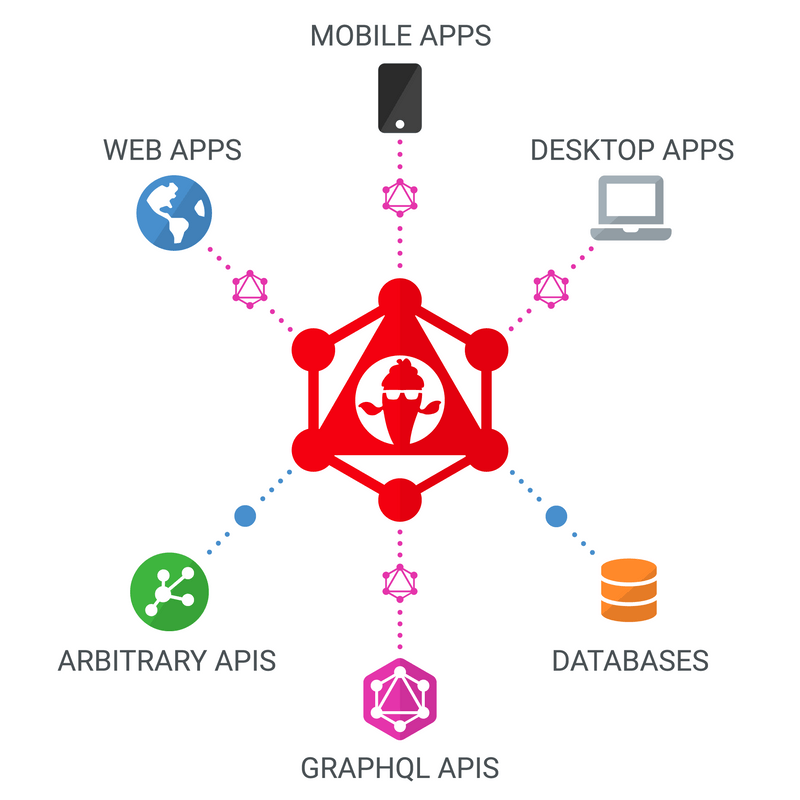
\includegraphics[width=0.6\linewidth]{images/hot_chocolate.png} 
	\caption{HotChocolate server}
	\label{slk:hot_chooclate}
\end{figure}
\FloatBarrier
\textcolor{red}{ADD IMAGE REFERENCE} https://chillicream.com/static/cfd2ddde71f95ed876541f87c15b2a08/78d47/platform.png\\https://chillicream.com/docs/hotchocolate/v13

\section{.NET i C\#}
.NET je otvorena platforma za razvoj raznih topova aplikacija (web-aplikacije, aplikacije za mobilne uređaje, video igre te drugo). Obuhvaća razne tehnologije i alate koji omogućavaju brzi razvoj aplikacija. Ključne komponente su .NET Runtime (zadužen za automatsko skupljanje smeća i upravljanje memorijom), .NET SDK (alati i biblioteke koje se koriste za razvoj .NET aplikacija, alati za \textcolor{red}{debuggiranje}) i .NET biblioteke (osnovne funkcionalnosti potrebne za razvoj aplikacija).
\\.NET okruženje podržava C\#, F\# i VB.NET jezike.
\\C\# je objektno orijentiran programski jezik dizajniran 2000. godine. Sintaksa C\# jezika je jednostavna te jezik omogućava izgradnju paralelnog koda što znatno ubrzava aplikacije. Često je uspoređivan s programskim jezikom Java.
\\Odabrane su ove tehnologije zbog jednostavnosti razvoja aplikacija u njima, te zbog toga što .NET podržava izvođenje i razvoj aplikacija na više platformi, uključujući i Windows i Linux.
\\Korištena .NET verzija: net8.0\\Korištena C\# verzija: 12.0
\begin{figure}[htb]
	\centering
	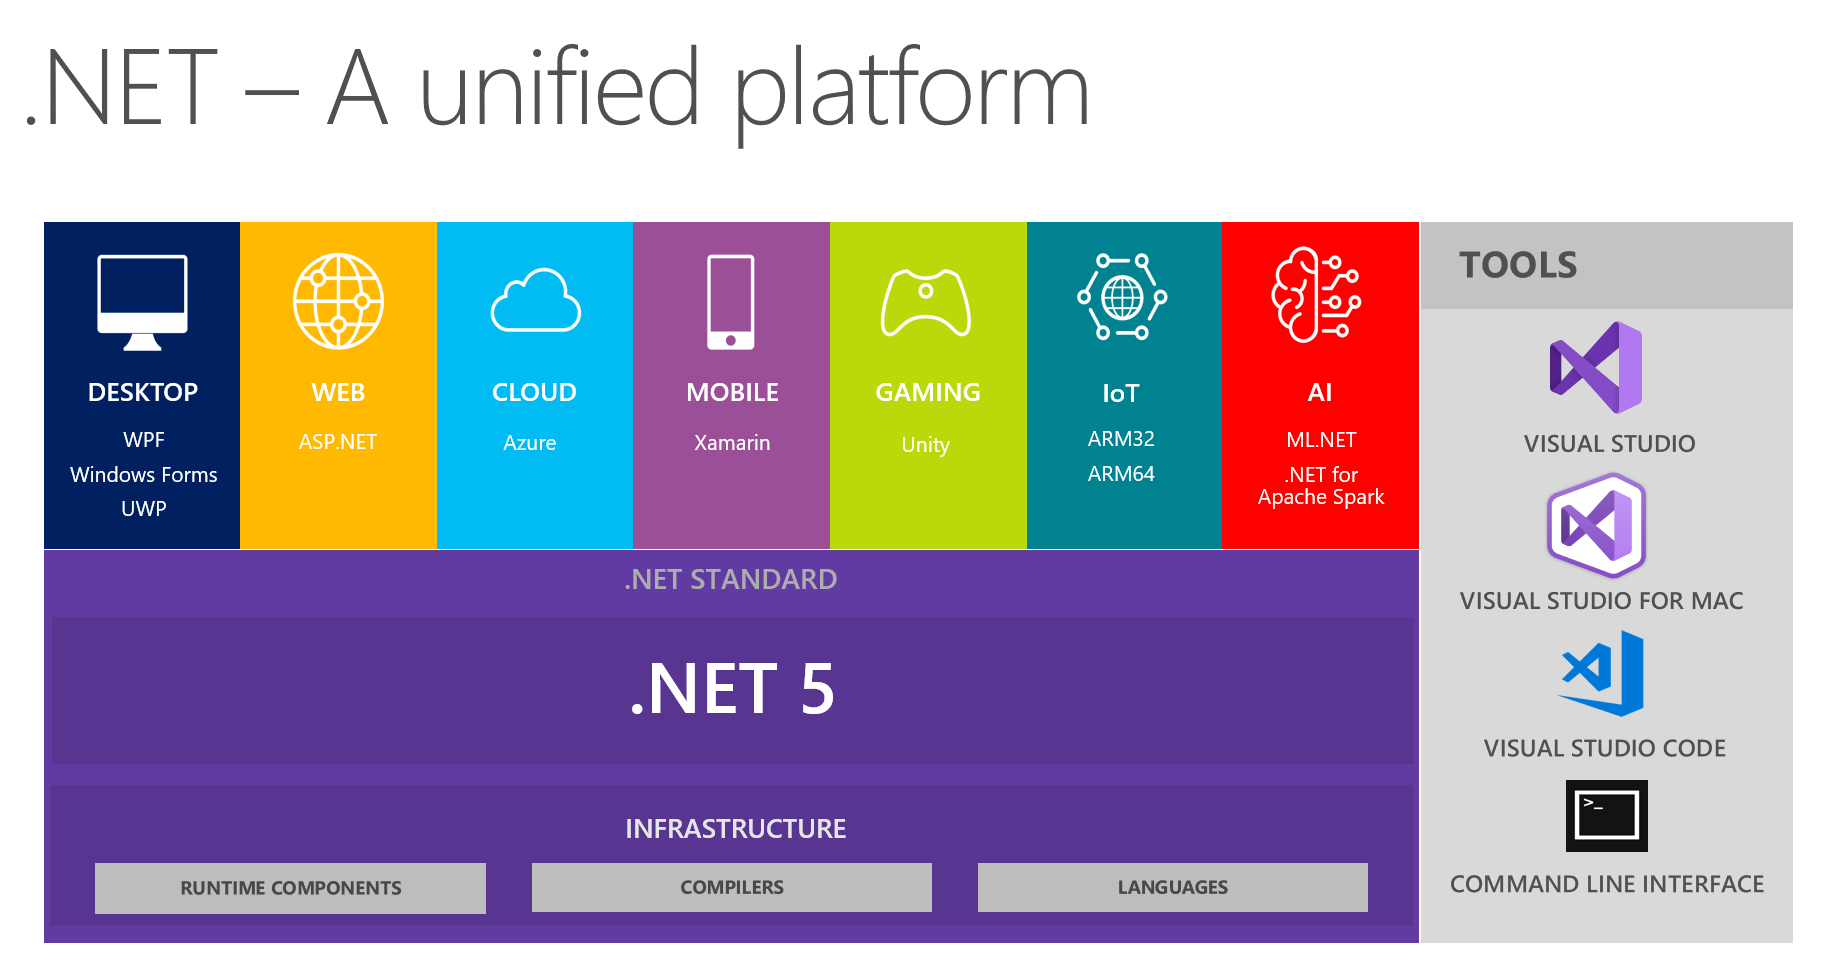
\includegraphics[trim={0 0 15cm 5cm},clip,width=1\linewidth]{images/dotnet5_platform.png} 
	\caption{Alati .NET platforme}
	\label{slk:dotnet}
\end{figure}
\FloatBarrier
\textcolor{red}{ADD IMAGE REFERENCE TO https://images.ctfassets.net/23aumh6u8s0i/2bsVrNvzMOk64yfFw0ZU3O/b88d3412d42844d54011f31d69d5860f/dotnet5\_platform}

\subsection{linq2db}
\label{pog:linq2db}
linq2db je .NET biblioteka koja se koristi za pretvaranje LINQ koda u SQL kod kako bi se moglo lako pristupati bazi podataka.
\\Nakon instalacije paketa se pomoću određenih naredbi može spojiti na bazu podataka i iz nje generirati C\# klase koje odgovaraju tablicama u bazi podataka:

\begin{figure}[htp]
	\centering
	\begin{lstlisting}[language=CSharp]
		using System;
		using LinqToDB.Mapping;
		
		[Table("Products")]
		public class Product
		{
			[PrimaryKey, Identity]
			public int ProductID { get; set; }
			
			[Column("ProductName"), NotNull]
			public string Name { get; set; }
			
			[Column]
			public int VendorID { get; set; }
			
			[Association(ThisKey = nameof(VendorID), OtherKey=nameof(Vendor.ID))]
			public Vendor Vendor { get; set; }
			
			// ... other columns ...
		}
	\end{lstlisting}
	\caption{Primjer linq2db koda}
\end{figure}
\FloatBarrier

linq2db repozitorij: \url{https://github.com/linq2db/linq2db}

\subsection{Newtonsoft.Json}
Newtonsoft.Json je C\# biblioterka koja se koristi za serijalizaciju i deserijalizaciju JSON podataka.
Newtonsoft.Json repozitorij: https://github.com/JamesNK/Newtonsoft.Json

\section{Vue.js}
\label{pog:vue}
Vue.js je Javascript razvojno okruženje koje se koristi za izradu korisničkog sučelja. Omogućava jednostavniji rad sa prikazom podataka i bolje strukturiranje koda od samog Javascript jezika.
\\Neke od prednosti Vue razvojnog okruženja:
\begin{itemize}
	\item \textit{progresivna arhitektura} - može se lako integrirati u postojeće projekte, te se nakon toga može postepeno proširivati
	\item \textit{komponente} - koriste se komponente kako bi se aplikacija razdvojila na manje, ponovno upotrebljive dijelove
	\item \textit{reaktivnost} - prikazani podaci se automatski osvježavaju kada se promijene varijable na koje su podaci vezani
	\item \textit{direktive} - Vue pruža direktive kao v-model, v-if, v-for te druge kako bi se jednostavno manipuliralo DOM-om
\end{itemize}

\textcolor{red}{Primjer Vue koda za povećanja vrijednosti gumba nakon klika (preuzeto sa \url{https://vuejs.org/guide/introduction.html}):}
\begin{figure}[htb]
	\centering
	\begin{lstlisting}[language=html]
		<div id="app">
		<button @click="count++">
		Count is: {{ count }}
		</button>
		</div>
	\end{lstlisting}
	\caption{Primjer Vue koda za povećanje gumba}
\end{figure}
\FloatBarrier

Korištena verzija: 3.2.13
\\Vue.js dokumentacija: \url{https://vuejs.org/guide/introduction.html}

\subsubsection{primevue}
Primevue sadržava razne Vue komponente koje se koriste za dinamički prikaz podataka na ekranu (prilikom promijene podataka se odmah mijenja i prikaz bez potrebe za dodatnim kodom). Također se koristi primeicons biblioteka koja omogućuje korištenje raznih ikona.
\\Korištena primevue verzija: 3.52.0
\\Korištena primeicons verzija: 7.0.0
\\Dokumentacija: \url{https://primevue.org/}

\subsubsection{vue-chartjs}
\label{pog:chart.vue}
Vue-chartjs Vue je biblioteka koja se koristi za vizualizaciju podataka ovisno o predanim parametrima. Omogućuje prikaz raznih tipova grafova kao linijski, stubičasti te točkasti graf koje se može konfigurirati kroz razne parametre.
\begin{figure}[htb]
	\centering
	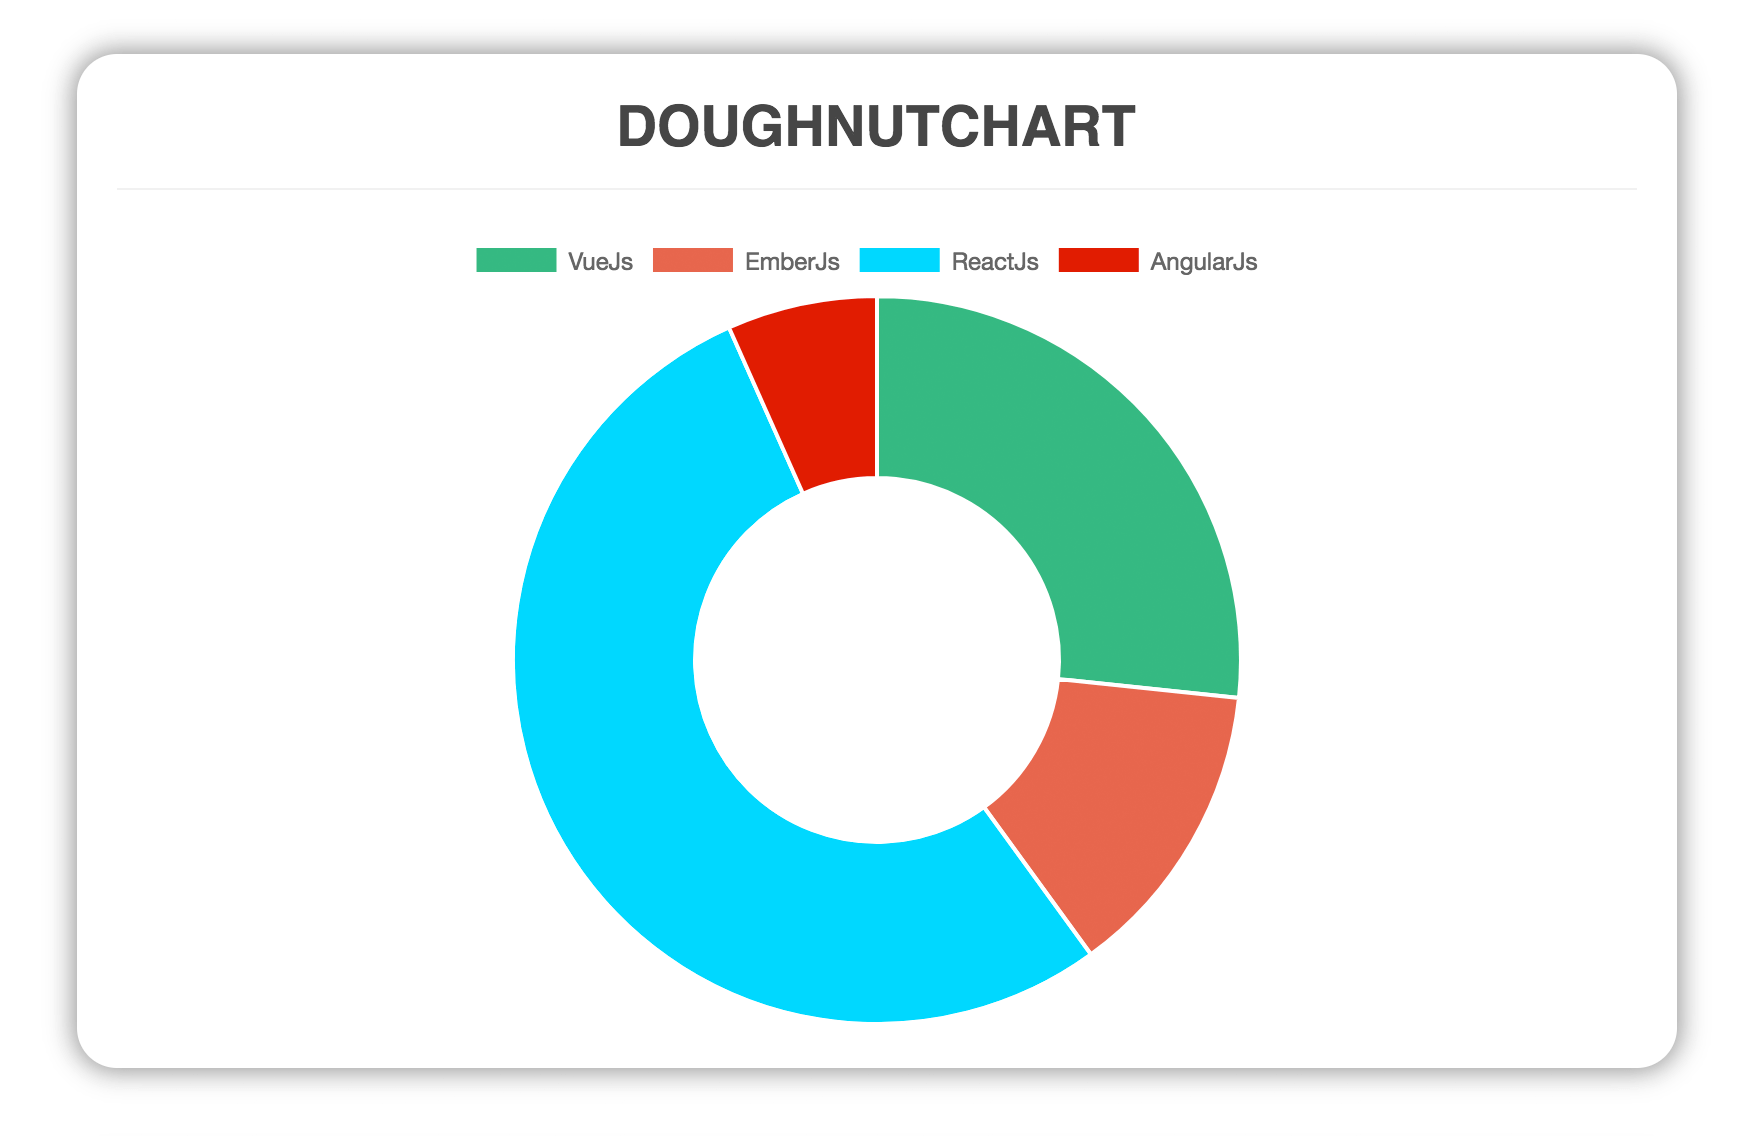
\includegraphics[width=0.9\linewidth]{images/chartjs_example.png} 
	\caption{Primjer chartjs grafa}
	\label{slk:chartjs_example}
\end{figure}
\FloatBarrier
\textcolor{red}{ADD IMAGE REFERENCE https://raw.githubusercontent.com/apertureless/vue-chartjs/HEAD/assets/doughnut.png}
\\Korištena verzija: 5.2.0
\\Dokumentacija: \url{https://vue-chartjs.org}

\subsubsection{vue-datepicker}
Vue-datepicker je Vue komponenta koja se koristi za odabir datuma i vremena. Klikom na komponentu se otvara kalendar na kojem korisnik može odabrati datum i vrijeme.
\begin{figure}[htb]
	\centering
	
\includegraphics[width=1\linewidth]{images/datepicker_example.png} 
	\caption{Primjer datepicker komponente}
	\label{slk:datepicker_example}
\end{figure}
\FloatBarrier
Korištena verzija: 7.1.0
\\Dokumentacija: \url{https://vue3datepicker.com/}

\section{PostgreSQL}
\label{pog:postgresql}
PostgreSQL relacijski je sistem za upravljanje bazama podataka (RDBMS) koji je otvorenog koda i besplatan. Poznat je po svojoj stabilnosti i fleksibilnosti.
\\Važne karakteristike PostgreSQL-a:
\begin{itemize}
	\item \textit{otvoreni kod} - PostgreSQL kod je otvorenog koda zbog čega bilo tko može vidjeti, izmijeniti i distribuirati
	\item \textit{moderni standardi} - implementira puno modernih karakteristika SQL jezika
	\item \textit{podrška za JSON} - omogućava rad sa JSON podacima, ukljućujući njihovu pohranu
	\item \textit{razni tipovi podataka} - podržava integer, varchar, boolean, array, uuid, xml te razne druge tipove podataka
	\item \textit{ACID (atomicity, consistency, isolation, durability)} - osigurava pouzdane transakcije i integritet podataka
\end{itemize}
Odabran je PostgreSQL kao RDBMS sustav za upravljanje bazom podataka zato što je otvorenog koda te ima opširnu dokumentaciju i korisničku podršku.
\\Korištena verzija: 16.2
\\PostgreSQL dokumentacija: \url{https://www.postgresql.org/docs}

\section{Git i Github}
Git je sustav za upravljanje kodom. Podržava verzioniranje datoteka što omogućava praćenje promijena koda te suradnju sa drugim programerima. Linus Torvalds napravio ga je 2005. godine te je danas jedan od najvažnijih alata za razvoj programa. Neke od važnijih karakteristika:
\begin{itemize}
	\item \textit{distributiranost} - svaki korisnik ima kompletnu kopiju repozitorija na svom računalu što omogućava rad na projektu kada korisnik nema pristup internetu
	\item \textit{verzioniranje datoteka} - omogućava praćenje promjena u datotekama kako se mijenjaju, što olakšava pronalazak koda koji je uzrokovao novu grešku
	\item \textit{grananje} - omogućava rad na odvojenim dijelovima projekta, neovisno o main/master grani
	\item \textit{rad u timu} - olakšava suradnju više programera koji svi rade na istom projektu pomoću raznih mehanizama, jedan od kojih je spriječavanje prebrisavanja koda kojeg je jedan programer objavio sa kodom kojeg drugi programer pokušava objaviti
\end{itemize}
Github je platforma za razvoj aplikacija temeljena na Git-u. Koristi se za lakše korištenje Git-a te pruža razne alate koji se mogu koristiti za organizaciju zadaća programerima.
\\Službena git stranica: \url{https://git-scm.com}
\\Github: \url{https://github.com/}


%-------------------------------------------------------------------------------
\chapter{Opis rješenja}
\label{pog:opis_rjesenja}
\section{\textcolor{red}{Softver}}
Napravljene su tri .NET projekta (API, Common i Monitor), web stranica te baza podataka.
\\API (programsko sučelje) je centralna aplikacija koja povezuje Monitor i web stranicu s bazom podataka. To je ostvareno pomoću GraphQL-a, kod kojeg se koristi Query objekt za dohvaćanje podatka za web stranicu, te Mutation objekti koji se koriste kako bi Monitor mogao pisati podatke u bazu podataka.
\\Monitor je aplikacija koja se pokreće na poslužitelju koji se prati. Ona u specificiranom intervalu prikuplja razne podatke o poslužitelju te ih šalje programsko sučelje koji ih zapisuje u bazu podataka.
\\Web stranica se zatim koristi za prikaz prikupljenih podataka o pojedinačnim serverima, te za prikaz obavijesti i upozorenja koje je programsko sučelje generiralo prilikom upisa podataka u bazu podataka.

\section{\textcolor{red}{Fizička konfiguracija}}
Postoji jedan centralni poslužitelj na kojem su pokrenute dvije aplikacije: Vue web stranica te programsko sučelje. Vue web stranica se dohvaća HTTP protokolom, nakon čega ona šalje zahtijeve programskom sučelju na centralnom poslužitelju radi dohvata podataka iz baze podataka.
\\Poslužitelji koji su konfigurirani za praćenje podataka također komuniciraju sa programskim sučeljem, ali ne za dohvaćanje nego za slanje podataka sučelju koji onda te podatke sprema u bazu podataka.
\begin{figure}[htb!]
	\centering
	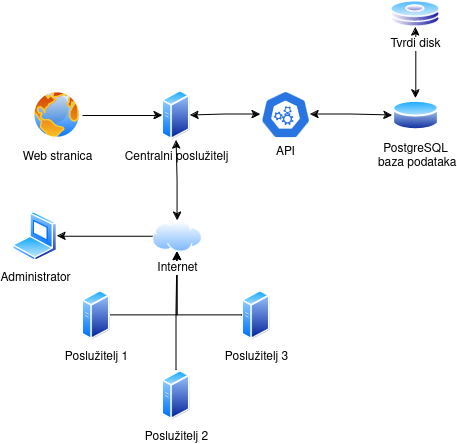
\includegraphics[width=0.6\linewidth]{images/flowchart.png} 
	\caption{Dijagram rješenja}
	\label{slk:flowchart}
\end{figure}
\FloatBarrier
U nastavku slijedi detaljan opis funkcionalnosti i koda svih projekata.

\chapter{Baza podataka}
Za izradu baze podataka je korišten \ref{pog:postgresql} Postgresql. U korijenskoj strukturi repozitorija se nalazi datoteka db.sql pomoću koje se stvara baza podataka. U nastavku je opisana struktura baze podataka.
\begin{figure}[htb!]
	\centering
	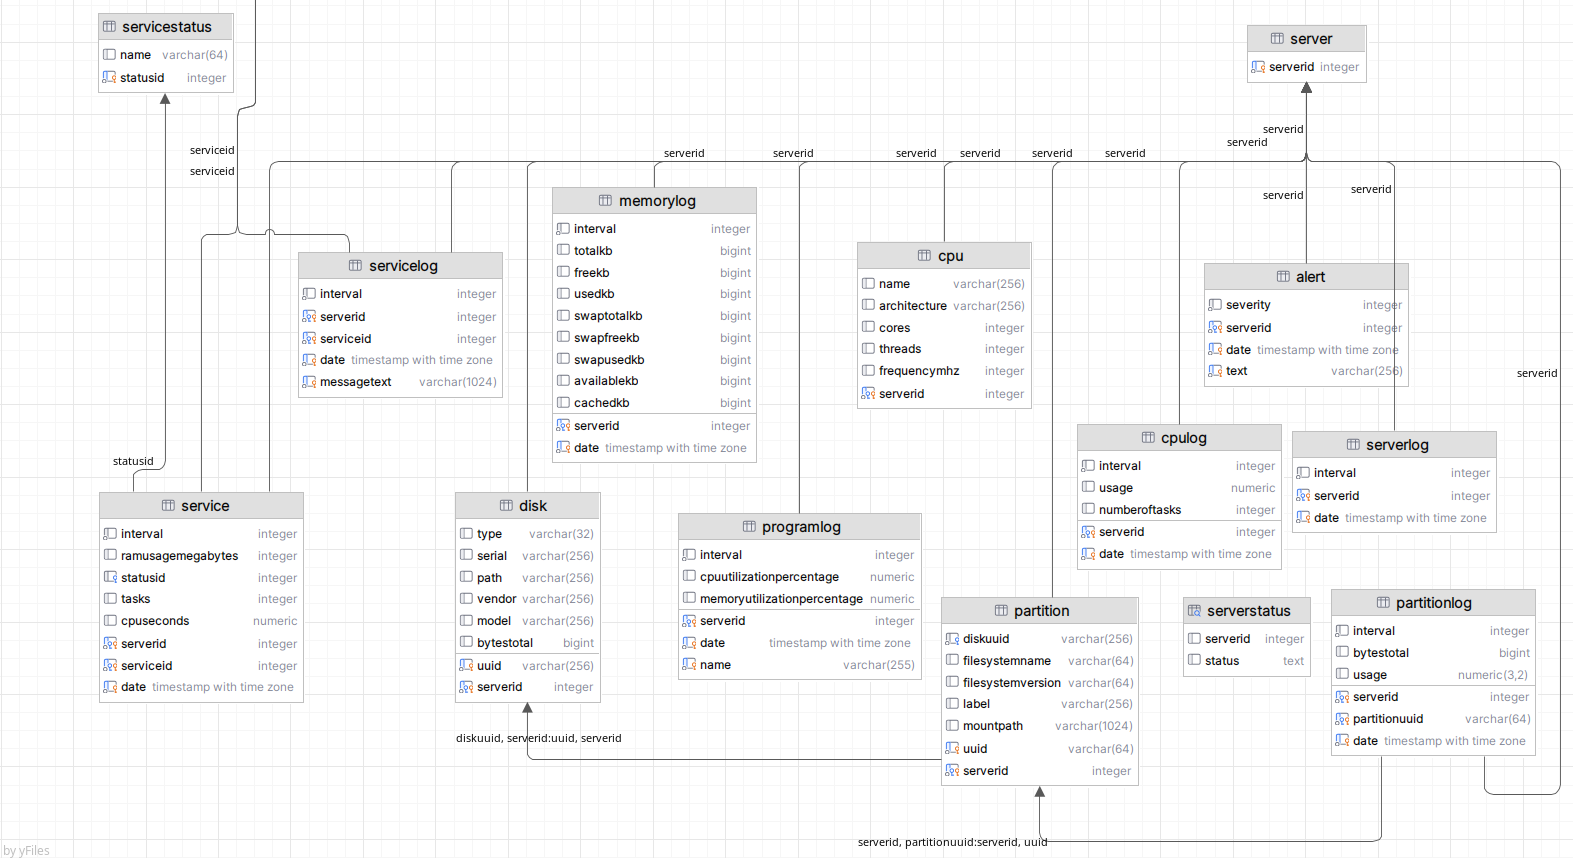
\includegraphics[width=1.4\linewidth,angle=90]{images/db_structure.png} 
	\caption{Struktura baze podataka}
	\label{slk:db_structure}
\end{figure}
\FloatBarrier

\section{Poslužitelj}
Za praćenje poslužitelja se koristi tablica server koja samo pohranjuje ID poslužitelja. Ovu tablicu referencira većina drugih tablica.
\\Također je napravljen jedan pogled koji se koristi za dohvat statusa poslužitelja. Poslužitelj se smatra aktivnim ako je od zadnjeg slanja podataka prošlo manje od n minuta (n = interval specificiran prilikom zadnjeg slanja podataka).

\begin{figure}[htb]
	\centering
	\lstinputlisting[firstline=16,lastline=22,language=SQL,label=]{db.sql}
	\caption{serverStatus pogled}
\end{figure}
\FloatBarrier

\section{Procesor}
Za praćenje podataka o procesoru se koriste tablice cpu i cpulog. Tablica cpu pohranjuje općenite podatke o procesoru: ime procesora (name), arhitektura (architecture), broj jezgri (cores), broj niti (threads), frekvencija rada (frequency) te poslužitelj kojem on pripada (serverId).
\\cpulog tablica sprema podatke o procesoru koji se mijenjaju tijekom vremena kao iskorištenost procesora (usage) i broj procesa koje on obrađuje (numberoftasks).

\section{Priručna memorija}
Za pohranjivanje podataka o priručnoj memoriji se koristi samo tablica memorylog koja pohranjuje podatke o datumu prikupljanja podataka (date) ukupnoj memoriji (totalkb, freekb, usedkb), "swap" memoriji (swaptotalkb, swapfreekb, swapusedkb), neiskorištenoj memoriji (availablekb), "cache" memoriji (cachedkb), te ID poslužitelja kojem memorija pripada.
\\Za razliku od procesora, ne koristi se zasebna tablica za pohranu općenitih podataka o priručnoj memoriji kao proizvođač, serijski broj te drugo, jer nije pronađen način da se ti podaci očitaju sa poslužitelja bez administratorskih privilegija.

\section{Trajna pohrana}
Za pohranu trajne memorije se koriste tablice:
\begin{itemize}
	\item disk - općenite informacije o tvrdom disku: jedinstveni ID (uuid), tip (type), serijski broj (serial), putanja na kojoj se disk nalazi (path), proizvođač (vendor), model, veličina diska (bytestotal) i ID poslužitelja na kojem se disk nalazi
	\item partition - općenite informacije o jednoj particiji: jedinstveni ID (uuid), UUID diska kojem pripada (diskuuid), tip i verzija datotečnog sustava (filesystemname, filesystemversion), naziv particije (label), putanja na kojoj se nalazi (mountpath) te ID poslužitelja na kojem se particija nalazi
	\item partitionlog - podaci o particiji koji se mijenjaju tijekom vremena kao veličina particije (bytestotal) te iskorištenost (usage)
\end{itemize}

\section{Servisi}
Servisi nisu do kraja implementirani u aplikaciji, no podloga za praćenje podataka o servisima je implementirana su u bazi podataka. Za praćenje servisa se koriste tablice:
\begin{itemize}
	\item service - prikupljeni podaci o statusu servisa kao pohrana koju koristi (ramusagemegabytes), broj procesa koje je servis stvorio (tasks), procesorska snaga koju koristi (cpuseconds) te status servisa (statusid)
	\item servicename - \textcolor{red}{mapira} jedinstveni broj u naziv servisa
	\item servicelog - pohranjuje poruke koje je servis poslao (messagetext) te vrijeme kada su poslane (date)
	\item servicestatus - \textcolor{red}{mapira} id statusa servisa u tekstualnu reprezentaciju
\end{itemize}

\section{Programi}
Podška za programe nije do kraja implementirana u aplikaciji, no podloga za njihovo praćenje je implementirana su u bazi podataka.
\\Za praćenje programa se koristi tablica programlog koji pohranjuje  neke podatke kao ime programa (name) te postotak procesora (cpuutilizationpercentage) i memorije (memoryutilizationpercentage) koju program koristi.

\section{Obavijesti}
Stvorena je tablica za obavijesti koja pohranjuje \textcolor{red}{kritičnost} poruke (severity), ID poslužitelja za koji je relevantna (serverid) te datum (date) i tekst poruke (text).
\\Uz tablicu je također napravljena i metoda before\_alert\_insert\_func() koja se poziva prije unosa podataka u tablicu. Metoda je stvorena kako bi se onemogućio unos iste obavijesti ako je ona već poslana u zadnjih sat vremena (na primjer ako se proba unijeti "Server 0 cpu load above 90\%" u razmaku od 30 minuta, ta poruka će biti zapisana samo prvi put u bazu podataka, a drugi put se odbacuje uz grešku).

\begin{figure}[htb]
	\centering
	\lstinputlisting[firstline=172,lastline=176,language=SQL]{db.sql}
	\caption{Metoda before\_alert\_insert\_func()}
\end{figure}
\FloatBarrier

\chapter{API}
API aplikacija je implementirana koristeći \ref{pog:hotchocolate} HotChocolate server paket koji implementira funkcionalnosti GraphQL poslužitelja.
\\Struktura projekta:
\begin{figure}[htb]
	\centering
	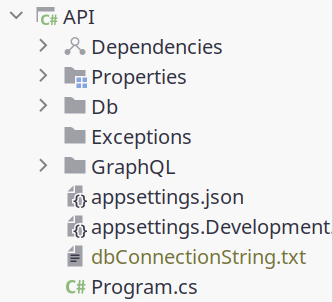
\includegraphics[width=0.4\linewidth]{images/api_structure.png} 
	\caption{Struktura API projekta}
	\label{slk:api_structure}
\end{figure}
\FloatBarrier

\section{Program.cs}
Program.cs je datoteka koja se pokreće prilikom pokretanja programa. Glavne funkcije koje ona izvršava su konfiguracija Dependency Injectiona te mapiranje putanja progamskog sučelja.
\\Dependency Injection je način strukturiranja koda kod kojeg se klase ne stvaraju direktno pomoću kodne riječi "new" nego se parametri konstruktora klase automatski predaju u nju. Odabran je ovaj način izrade koda kako bi se omogućilo lagano testiranje koda u budućnosti jer se umjesto stvarne klase koja obavlja određenu funkcionalnost može predati lažna klasa koja emulira stvarnu klasu (na primjer kao "IDb database" sučelje se umjesto klase koja obavlja funkcionalnolsti stvarne baze podataka predaje lažna klasa koja samo provjerava da li je određena metoda pozvana tri puta; ako da onda je test ispravan a u suprotnom je neispravan).

\section{GraphQL direktorij}
\label{pog:graphql_dir}
GraphQL direktorij sadržava sav kod potreban za ispravan rad GraphQL poslužitelja kao Query i Mutation kodovi te kod za rad sa obavijestima.

\begin{figure}[htb!]
	\centering
	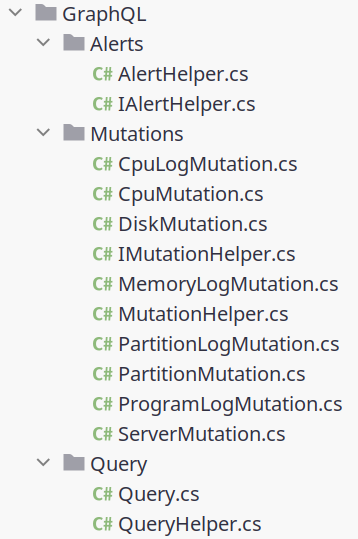
\includegraphics[width=0.5\linewidth]{images/graphql_dir_structure.png} 
	\caption{Struktura GraphQL direktorija}
\label{slk:graphql_dir_structure}
\end{figure}
\FloatBarrier

\subsection{Query.cs}
\label{pog:query.cs}
Koristi se za dohvat podataka iz baze podataka. Za svaki tip podatka (CPU, memorija, tvrdi disk, ...) je napravljena metoda koja se poziva kada korisnik šalje zahtjev pomoću kojega se pokušava dohvatiti određen podatak.
\\Svaka metoda predstavlja tip query objekta koji se pokušava dohvatiti, a svi parametri te metode predtavljaju argumente koje korisnik specificira tijekom slanja zahtjeva.
\\Neki od parametara koje gotova svaka metoda ima su:
\begin{itemize}
	\item serverId - dohvaćaju se samo podaci koje je poslao server čiji je ID jednak ovom argumentu
	\item startDateTime - dohvaćaju se samo podaci poslani nakon specificiranog datuma i vremena
	\item endDateTime - dohvaćaju se samo podaci poslani prije specificiranog datuma i vremena
\end{itemize}
Klasa se oslanja na \ref{pog:db_dir} IDbProvider sučelje za rad sa bazom podataka, te na metodu \ref{GetLogs} GetLogs metodu za dohvat \textcolor{red}{logova} iz baze podataka.
\\Primjer jedne takve metode:
\begin{figure}[htb]
	\centering
	\lstinputlisting[language=CSharp, firstline=21, lastline=48]{API/GraphQL/Query/Query.cs}
	\caption{Cpu metoda}
\end{figure}
\FloatBarrier

\subsection{QueryHelper.cs}
Pomoćna klasa koju koristi \ref{pog:query.cs} Query.cs klasa. Sastoji se od raznih metoda od kojih je najbitnija GetLogs metoda koja sadržava algoritam koji se koristi za spajanje više podataka u jedan. Algoritam radi tako da pomoću početnog i zadnjeg datuma izračuna interval unutar kojeg se podaci spajaju u jedan:

\begin{figure}[htb]
	\centering
	\begin{lstlisting}[language=CSharp]
		return (int)((DateTime)endDate).Subtract((DateTime)startDate).TotalHours;
	\end{lstlisting}
	\caption{Izračun intervala}
\end{figure}
\FloatBarrier

Nakon izračuna intervala se dohvačaju podaci iz tablice koji su pohranjeni nakon specificiranog početnog datuma i prije krajnjeg datuma. Nakon toga se prolazi kroz svaki podatak te se koristi \ref{pog:dataset_helper} DatasetHelper klasa za spajanje više podataka u jedan, te se na kraju list spojenih podataka vraća.

\begin{figure}[htb]
	\centering
	\lstinputlisting[language=CSharp, firstline=99, lastline=105]{API/GraphQL/Query/QueryHelper.cs}
	\caption{Parametri GetLogs metode}
\end{figure}
\FloatBarrier

\subsection{DatasetHelper.cs}
\label{pog:dataset_helper}
Pomoćna klasa korištena u algoritmu spajanja više podataka u jedan podatak. Najvažnija metoda u klasi je AddLog metoda koja dodaje podatak u listu podataka koja se kasnije vraća. Broj podataka koji se spaja u jedan podatak ovisi o intervalu. Na primjer ako je interval 30, a podaci se bilježe svakih 5 minuta, spaja se 6 podataka u jedan. Ako je došlo do prekida u slanju podataka (na primjer podaci se šalju svakih 5 minuta, ali jedan podatak se pošalje nakon 7 minuta), onda se za period između ta dva podatka vraća "prazan" podatak koji signalizira prekid u slanju podataka. Algoritam radi na ovaj način kako bi se korisnike moglo obavijestiti ukoliko je došlo do prekida slanja podataka.

\begin{figure}[htb]
	\centering
	\lstinputlisting[language=CSharp, firstline=20, lastline=50]{API/GraphQL/Query/DatasetHelper.cs}
	\caption{Metoda AddLog}
\end{figure}
\FloatBarrier

\subsection{Mutations direktorij}
Sadržava klase i sučelja koja se koriste za dodavanje i osvježavanje podataka u bazi podataka.
\\Važnije klase i sučelja u direktoriju:
\begin{itemize}
	\item IMutationHelper - sučelje koje definira funkcionalnosti koje su potrebne za umetanje, osvježavanje i brisanje pojedinačnih ili liste podataka iz baze podataka
	\item MutationHelper - implementacija IMutationHelper sučelja
\end{itemize}

Primjer dijela jedne mutacije:
\begin{figure}[htb]
	\centering
	\lstinputlisting[language=CSharp, firstline=10, lastline=24]{API/GraphQL/Mutations/CpuMutation.cs}
	\caption{Dio CpuMutation mutacije}
\end{figure}
\FloatBarrier

\subsection{IAlertHelper.cs}
Koristi se za slanje obavijesti bazi podataka. Poruka se odbacuje ukoliko je ista poruka za isti poslužitelj već poslana prije manje od sat vremena.

\begin{figure}[htb]
	\centering
	\lstinputlisting[language=CSharp, firstline=5]{API/GraphQL/Alerts/IAlertHelper.cs}
	\caption{IAlertHelper.cs sučelje}
\end{figure}
\FloatBarrier

\section{Db direktorij}
\label{pog:db_dir}
Db direktorij sadržava sve pomoćne klase i modele koji se koriste za interakciju sa bazom podataka. Većina klasa u direktoriju Models su automatski generirane (i djelomično ručno promijenjene) korištenjem \ref{pog:linq2db} linq2db paketa pomoću naredbe "dotnet linq2db scaffold -p PostgreSQL -c "Host=localhost; Username=[username];\\Password=[password];Database=[database]""

\begin{figure}[htb!]
	\centering
	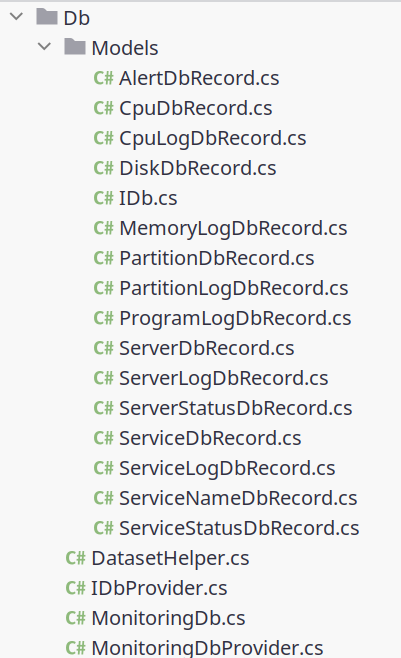
\includegraphics[width=0.5\linewidth]{images/db_dir_structure.png} 
	\caption{Struktura Db direktorija}
	\label{slk:db_dir_structure}
\end{figure}
\FloatBarrier

Neke od važnijih klasa (te one koje nisu automatski generirane):
\begin{itemize}
	\item Models/IDb.cs - sučelje koje sadržava popis svih tablica u bazi podataka
	\begin{figure}[htb]
		\centering
		\lstinputlisting[language=CSharp,firstline=6]{API/Db/Models/IDb.cs}
		\caption{IDb sučelje}
	\end{figure}
	\FloatBarrier
	\item MonitoringDb.cs - automatski generirana implementacija IDb.cs sučelja
	\item MonitoringDbProvider.cs - koristi se za generiranje nove konekcije na bazu podataka (potrebno jer se koristi Dependency Injection)
\end{itemize}

\section{Konfiguracijske datoteke}
U programu se nalaze tri konfiguracijske datoteke: appsetting.json, appsettings.Development.json i dbConnectionString.txt od kojih će samo zadnja biti opisana.
\\dbConnectionString.txt datoteka sadržava niz znakova koji se koristi za spajanje na postojeću bazu podataka prilikom pokretanja programa:
\begin{figure}[htb]
	\centering
	\begin{lstlisting}
		Host=localhost;Username=[username];Password=[password];Database=[dbName];Include Error Detail=[true for debugging; false for deployment]
	\end{lstlisting}
	\caption{Primjer datoteke dbConnectionString.txt}
\end{figure}
\FloatBarrier

\section{Pokretanje progamskog sučelja}
API se pokreće iz komandne linije/terminala pomoću naredbe "dotnet run" unutar direktorija u kojem se aplikacija nalazi.
\\Nakon pokretanja se može pristupiti URL-u \url{http://localhost:3000//graphql}, prilikom čega se otvara web stranica na kojoj se može vidjeti dokumentacija programskog sučelja te se mogu izvršavati upiti.
\begin{figure}[htb!]
	\centering
	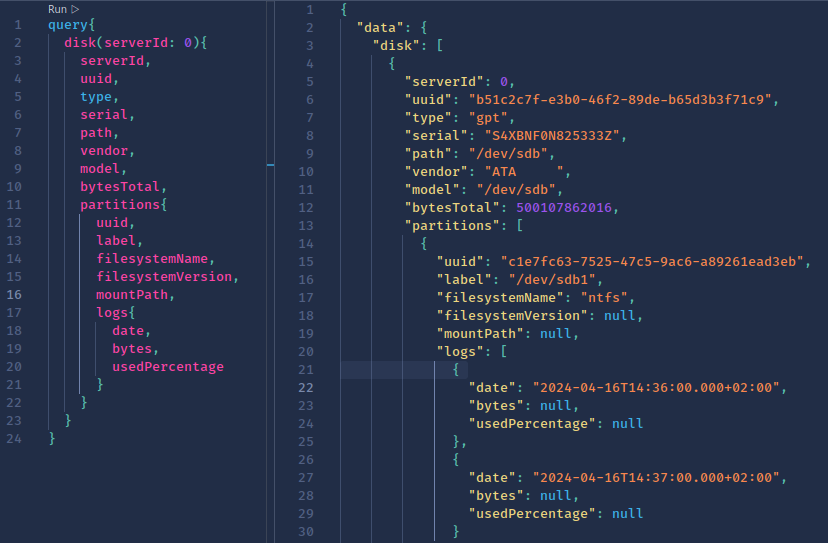
\includegraphics[width=1\linewidth]{images/api_query.png} 
	\caption{Dohvat podataka o pohrani}
	\label{slk:api_query}
	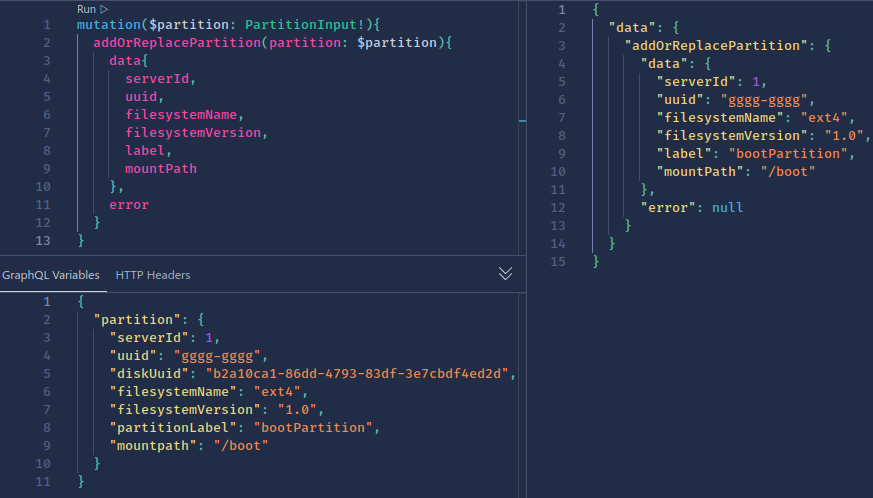
\includegraphics[width=1\linewidth]{images/api_mutation.png} 
	\caption{Dodavanje jedne particije}
	\label{slk:api_mutation}
\end{figure}
\FloatBarrier

\chapter{Monitor}
Aplikacija Monitor se koristi za prikupljanje podataka o poslužitelju te slanje tih podataka programskom sučelju.

\begin{figure}[htb!]
	\centering
	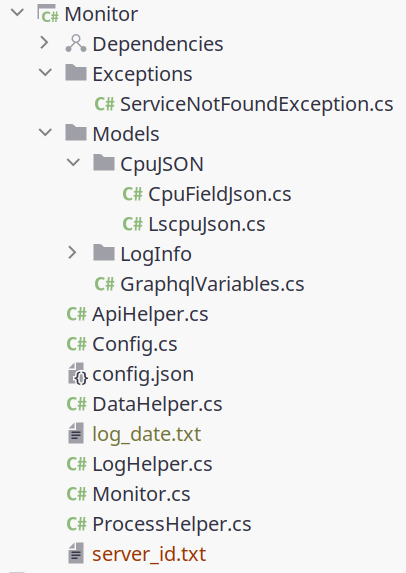
\includegraphics[width=0.4\linewidth]{images/monitor_structure.png} 
	\caption{Struktura Monitor projekta}
	\label{slk:monitor_structure.png}
\end{figure}
\FloatBarrier

Objašnjenje važnijih dijelova aplikacije:
\begin{itemize}
	\item Monitor.cs - pokreće se prilikom pokretanja aplikacije
	\item Models direktorij - sadržava klase koje se koriste za serijalizaciju i deserijalizaciju podataka dohvaćenih sa terminala
	\item ApiHelper.cs - koristi se za slanje podataka programskom sučelju
	\item config.json - koristi ju korisnik kako bi konfigurirao aplikaciju
	\item DataHelper.cs - čita podatke sa terminala te ih deserijalizira u klase koje se nalaze u Models direktoriju
	\item LogHelper.cs - pokreće proces dohvaćanja podataka svakin [n] minuta (n = definiran u config.json datoteci)
	\item ProcessHelper.cs - koristi se za pokretanje procesa u terminalu
\end{itemize}

\section{Monitor.cs}
Pokreće se prilikom pokretanja aplikacija. Na početku učitava konfiguracijsku datoteku, te zatim generira nasumični broj za ID poslužitelja. Na kraju se u beskonačnoj petlji pokreće proces prikupljanja podataka te slanje tih podataka programskom sučelju.

\begin{figure}[htb]
	\centering
	\lstinputlisting[firstline=10,lastline=30,language=CSharp]{Monitor/Monitor.cs}
	\caption{Glavna metoda programa Monitor}
\end{figure}
\FloatBarrier

\chapter{Common}
Projekt Common sadržava klase i sučelja koje koristi više projekata. Stvoren je kako bi se izbjeglo ponavljanje koda. Neke od važnijih klasa i sučelja:
\begin{figure}[htb!]
	\centering
	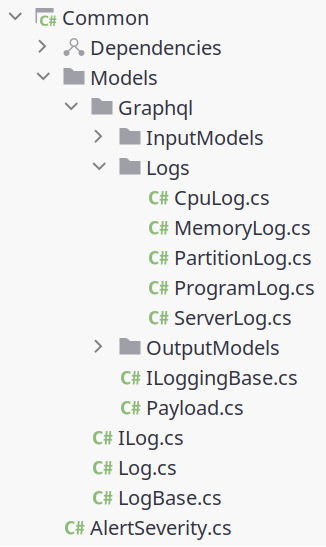
\includegraphics[width=0.4\linewidth]{images/common_structure.png} 
	\caption{Struktura Common projekta}
	\label{slk:common_structure.png}
\end{figure}
\FloatBarrier

\section{ILog.cs}
Glavno sučelje, svaki Log nasljeđuje polja definirana u njemu.
\begin{figure}[htb]
	\centering
	\lstinputlisting[firstline=3,language=CSharp]{Common/Models/ILog.cs}
	\caption{ILog sučelje}
\end{figure}
\FloatBarrier

\section{Graphql direktorij}
Graphql direktorij sadržava klase i sučelja koji se koriste za komunikaciju API i Monitor programa.
Neko od važnijih komponenti direktorija:
\begin{itemize}
	\item Payload.cs - sastoji se od Data polja koje sadržava podatke o poslužitelju koji se vraćaju korisniku te Error polja koje je prazno osim u slučaju pogreške prilikom obrade zahtjeva
	\item InputModels direktorij - sadržava klase koje se koriste prilikom dodavanja ili izmijene podataka. Primjer klase:
	\begin{figure}[htb]
		\centering
		\lstinputlisting[firstline=3,language=CSharp]{Common/Models/Graphql/InputModels/CpuInput.cs}
		\caption{CpuInput klasa}
	\end{figure}
	\FloatBarrier
	\item Logs direktorij - sadržava klase koje opisuju Log podatke za određen aspekt poslužitelja
	\item OutputModels direktorij - sadržava klase koje se koriste prilikom vraćanja API odgovora. Primjer klase:
	\begin{figure}[htb]
		\centering
		\lstinputlisting[firstline=5,language=CSharp]{Common/Models/Graphql/OutputModels/MemoryOutput.cs}
		\caption{MemoryOutput klasa}
	\end{figure}
	\FloatBarrier
\end{itemize}

\chapter{Web stranica}
Web stranica je napravljena pomoću \ref{pog:vue} Vue razvojne okoline. Sastoji se od raznih kompoennti koje se koriste za prikaz i dohvaćanje podataka od programskog sučelja.
Koristi se Vue razvojna okolina te se zbog toga koristi samo jedna HTML stranica koja se nalazi u direktoriju "public". Stranica se koristi kao kostur web-stranice u kojem se prikazuju renderirane komponente.

\section{App.vue}
Glavna Vue komponenta koja kontrolira sadržaj koji se prikazuje, stvara se prilikom pokretanja programa.
\\Na početku komponente se nalazi glavni izbornik koji koristi \textit{Vue router} komponentu koja renderira određenu komponentu, ovisno o tome na kojoj putanji se korisnik nalazi. Kod za prikaz izbornika je preuzet sa službene Vue dokumentacije te je djelomično izmijenjen:
\begin{figure}[htb]
	\centering
	\lstinputlisting[firstline=50, lastline=69, language=HTML]{website/src/App.vue}
	\caption{Kod za prikaz izbornika}
\end{figure}
\FloatBarrier
Prilikom stvaranja komponente se šalje upit programskom sučelju kako bi se dohvatila i popunila lista poslužitelja, te se zatim korisnik prosljeđuje na putanju prikaza podataka prvog poslužitelja (osim ako nisu zabilježeni podaci za bilo koji poslužitelj).

\section{Vue komponente}
Vue razvojna okolina koristi komponente kako bi se dijelovi koda mogli ponovno koristiti. Sve korištene komponente se nalaze u direktoriju \textit{components}.

\subsubsection{Komponenta Chart}
Komponenta \textit{Chart} se koristi za prikaz linijskog grafa.
\\Parametri komponente:
\begin{itemize}
	\item \textit{name} - naslov grafa
	\item \textit{chartData} - točke grafa
	\item \textit{scales} - konfiguracijsko polje za x i y osi
\end{itemize}
Koristi nekoliko pomoćnih polja za ispravan rad, od kojih je najvažnije polje \textit{options} koje omogućava pregled uvećanje grafa, postavlja x os kao vremensku od i y os kao brojčanu os, te pokreće \textit{emitZoomChanged} događaj.
\\Komponenta koristi \textit{emitZoomChanged} događaj kako bi roditelju javila da je graf uvećan, što je potrebno kako bi roditelj mogao osvježiti za taj period vremena i poslati ih ih komponenti.


\subsubsection{Ostale komponente}
Komponente \textit{CpuInfo}, \textit{DiskInfo} i \textit{MemoryInfo} se koriste za prikaz podataka o procesoru i pohrani. Komponente rade na sličan način:
\begin{itemize}
	\item komponenti se mogu predati parametri \textit{startDate} (specificira početni datum grafa), \textit{endDate} (završni datum grafa) i \textit{serverId} (ID poslužitelja na kojeg se komponenta odnosi)
	\item nakon kreiranja komponente se učitavaju podaci pomoću \textit{Api} klase te se ti podaci pretvaraju u podatke povoljne za prikaz grafom pomoću \textit{ChartHelper} klase
	\item podaci se prikazuju pomoću \textit{Fieldset} komponente na čijem početku se nalaze generalni podaci o komponente te ispod toga graf (ili grafovi)
	\item nakon primanja događaja \textit{zoomChanged} od grafa, podaci za taj graf se ponovno učitavaju za novi period grafa
\end{itemize}
Primjer dijela jedne takve komponente:
\begin{figure}[htb]
	\centering
	\lstinputlisting[language=Javascript,firstline=53]{website/src/components/MemoryInfo.vue}
	\caption{Dio MemoryInfo komponente}
\end{figure}
\FloatBarrier

\section{Direktorij models}
Direktorij Models sadržava razne klase koje se koriste za pohranjivanje podataka dohvaćenih s programskog sučelja.
\\Primjer modela:
\begin{figure}[htb]
	\centering
	\lstinputlisting[firstline=3,language=Javascript]{website/src/models/Partition.ts}
	\caption{Model particije}
\end{figure}
\FloatBarrier

\section{Klasa Api}
Klasa Api je zadužena za komunikaciju s programskim sučeljem.
\\Primjer dohvaćanja podataka o poslužiteljima:
\begin{figure}[htb]
	\centering
	\lstinputlisting[firstline=161,language=Javascript]{website/src/api.ts}
	\caption{Dohvaćanje podataka o poslužiteljima}
\end{figure}
\FloatBarrier

\section{ChartHelper.ts}
Pomoćna datoteka koja se koristi za pretvorbu podataka koje programsko sučelje vraća u točke na grafu. Metode ove klase prolaze kroz \textit{logs} parametar te za svaki podataka vraćaju podatke relevantne za graf.
\\Primjer metode koja vraća točke za graf particije:
\begin{figure}[htb]
	\centering
	\lstinputlisting[firstline=102,language=javascript]{website/src/ChartHelper.ts}
	\caption{Vraćanje točaka grafa za podatke particije}
\end{figure}
\FloatBarrier

\chapter{Korisničko sučelje i interakcija}
Otvaranjem web-stranice se prikazuje glavna stranica. Na njoj se prikazuje izbornik sa listom poslužitelja i karticom za obavijesti. Ukoliko barem jedan poslužitelj postoji, prikazuju se podaci o prvom poslužitelju.
\begin{figure}[htb]
	\centering
	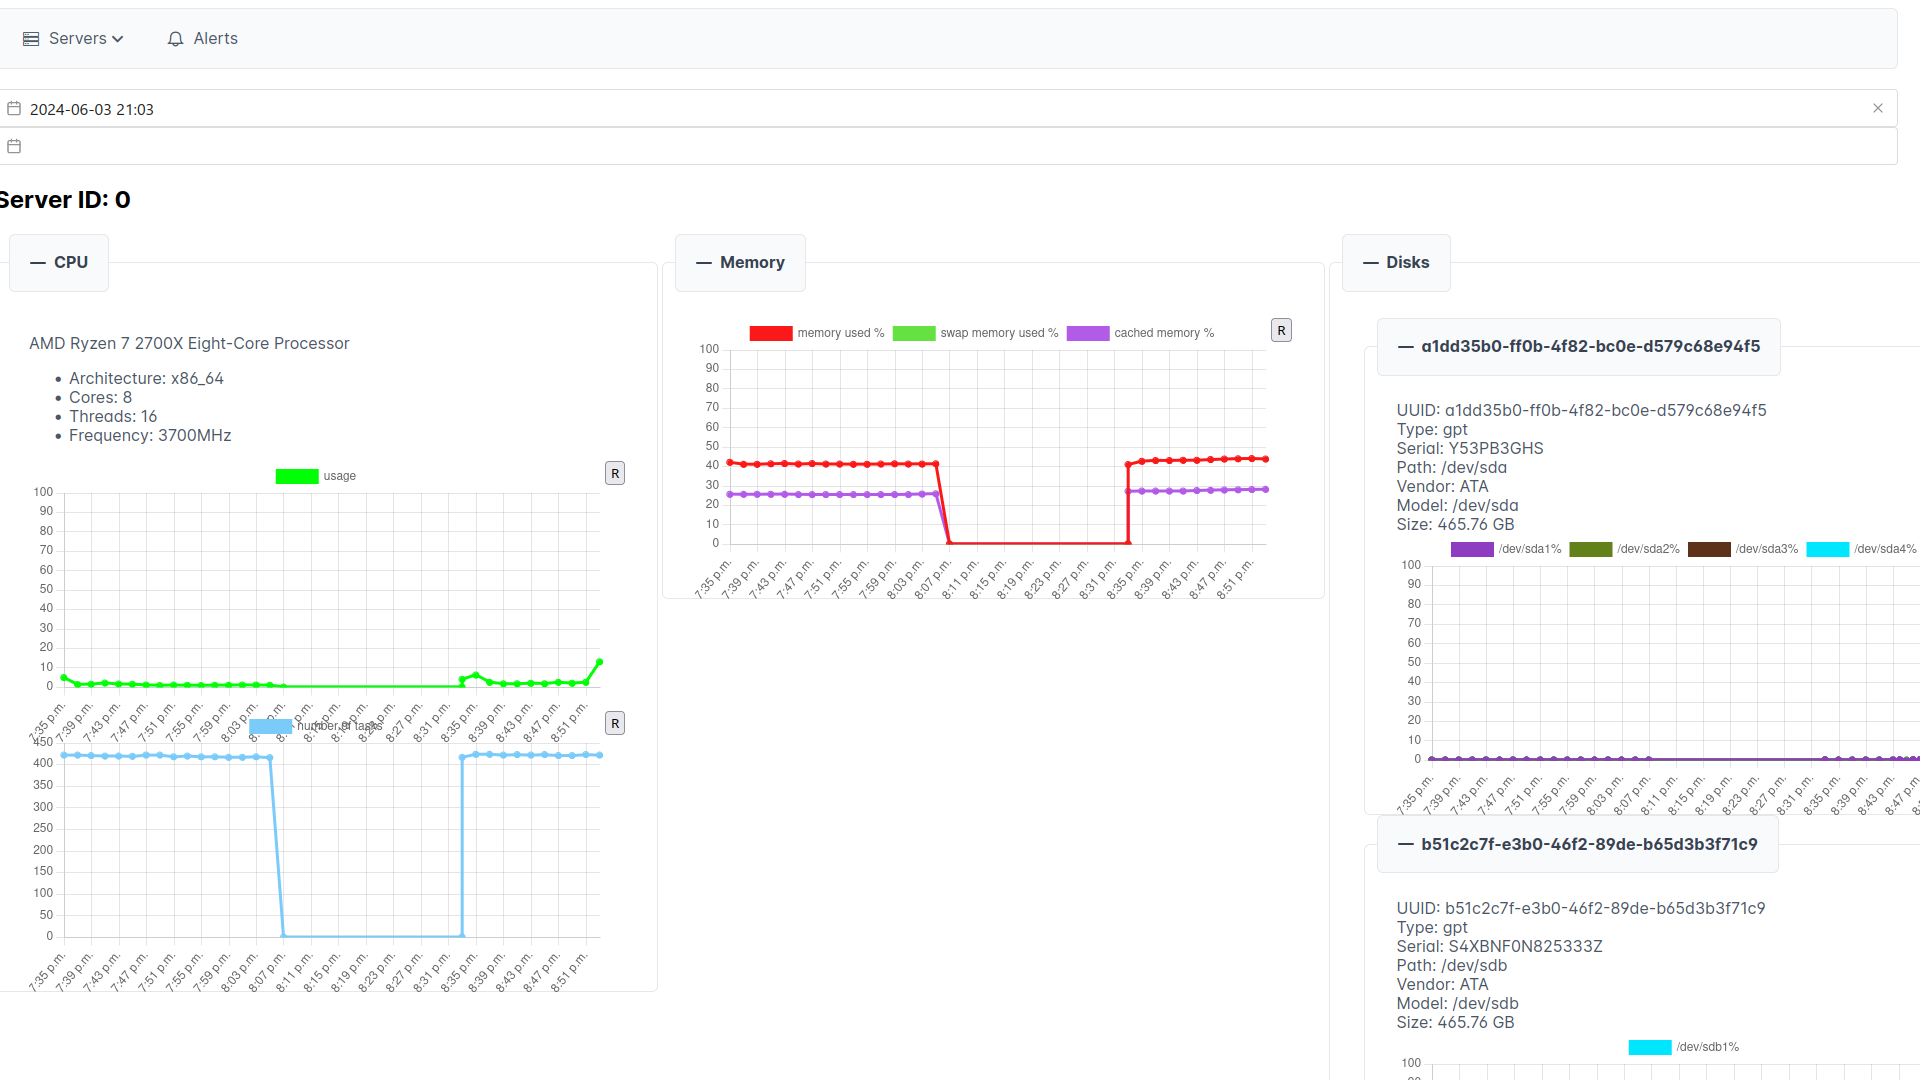
\includegraphics[width=1\linewidth]{images/web_1.png} 
	\caption{Početna stranica}
\end{figure}
\FloatBarrier
Moguće je odabrati početni i završni datum, čijim mijenjanjem se osvježavaju svi podaci web stranice.
\begin{figure}[htb]
	\centering
	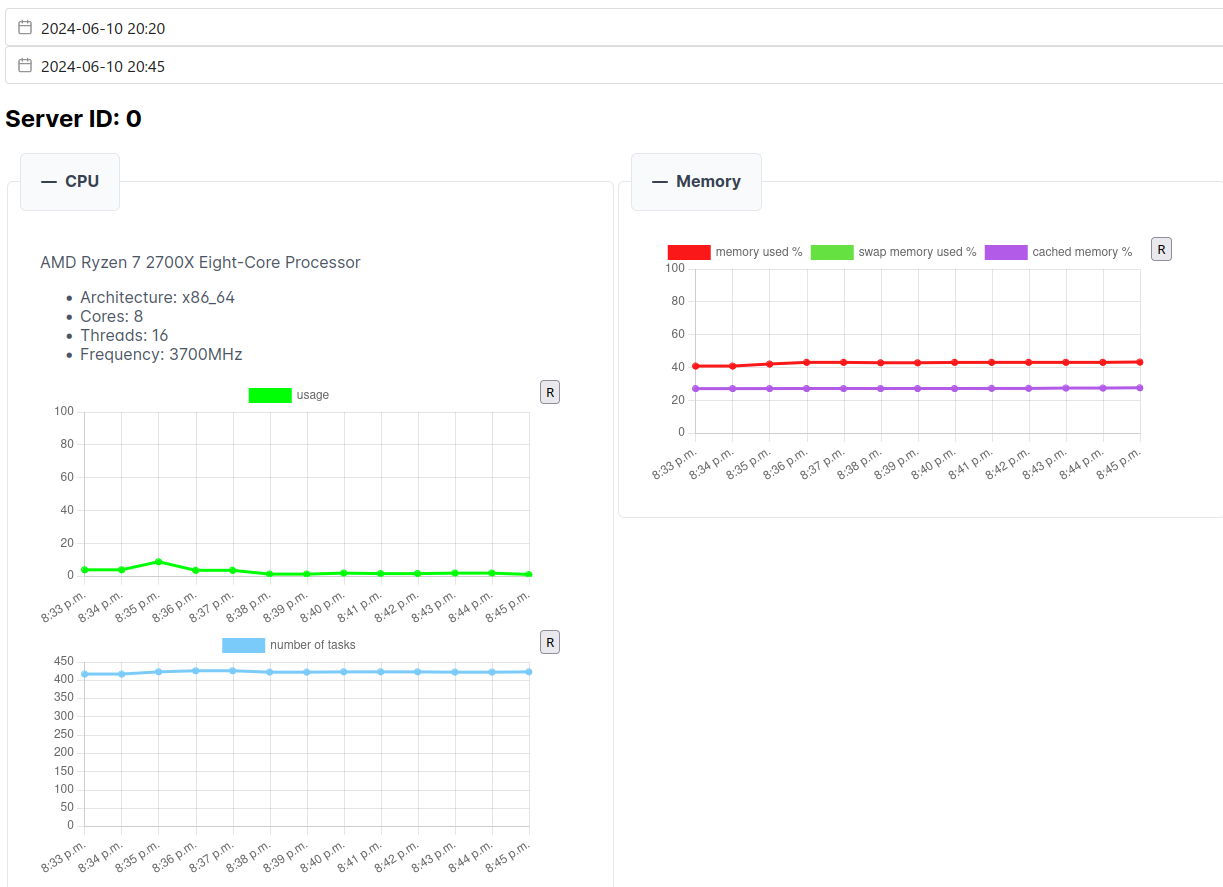
\includegraphics[width=1\linewidth]{images/web_2.png} 
	\caption{Početna stranica sa filtriranim datumom}
\end{figure}
\FloatBarrier
Prilikom učitavanja podataka za graf se prikazuje poruka \textit{Loading...}, a u slučaju da podataka nema se prikazuje \textcolor{red}{\textit{No data...}}

Pojedinačne grafove je moguće uvećati čime se osvježavaju podaci. Graf je također moguće \textcolor{red}{resetirati} čime se osvježavaju podaci za originalni period.
\begin{figure}[htb]
	\centering
	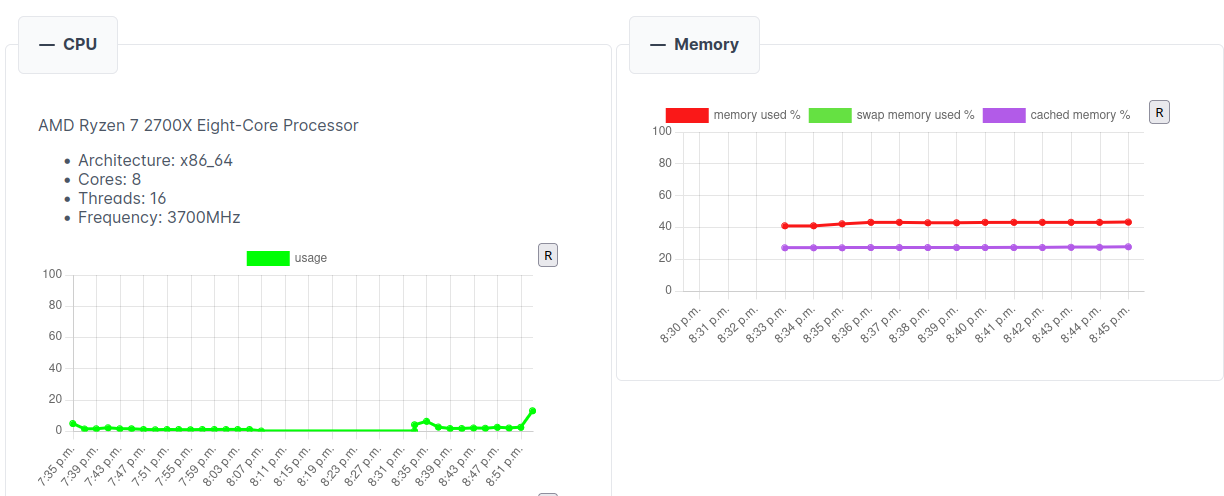
\includegraphics[width=1\linewidth]{images/web_3.png} 
	\caption{Primjer uvećanja grafa \textit{Memory}}
\end{figure}
\FloatBarrier

Kartice komponenti je moguće smanjiti čime se mijenja izgled stranice (proširuju se komponente kako bi stale na ekran).
\begin{figure}[htb]
	\centering
	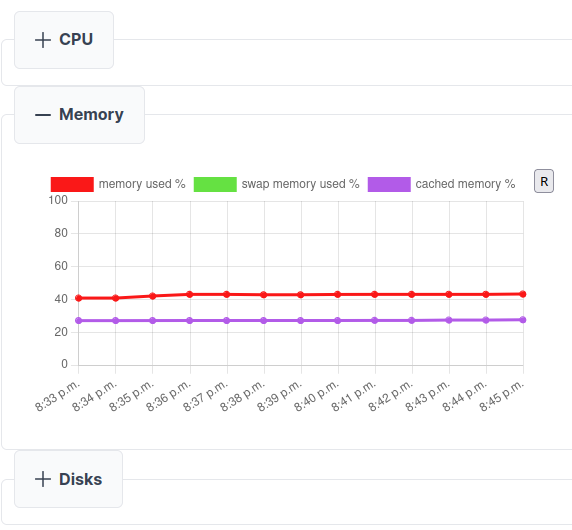
\includegraphics[width=0.75\linewidth]{images/web_4.png} 
	\caption{Izgled web-stranice nakon umanjena kartica}
\end{figure}
\FloatBarrier

Klikom na karticu \textit{Alerts} se prikazuju obavijesti i upozorenja.
\begin{figure}[htb]
	\centering
	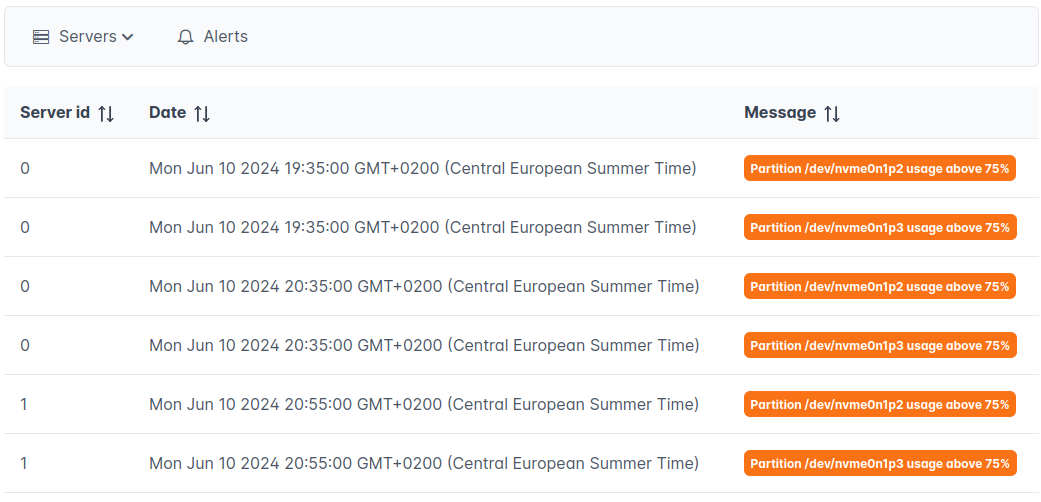
\includegraphics[width=0.9\linewidth]{images/web_5.png} 
	\caption{Prikaz obavijesti i upozorenja}
\end{figure}
\FloatBarrier

Web-stranica podržava široke ekrane te mobilne uređaje.
\begin{figure}[htb]
	\centering
	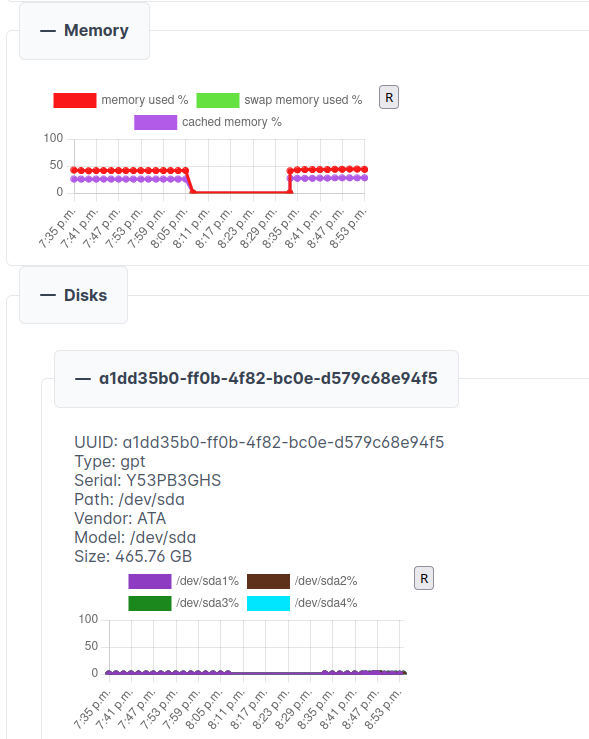
\includegraphics[width=0.75\linewidth]{images/web_6.png} 
	\caption{Web-stranica na mobilnim uređajima}
\end{figure}
\FloatBarrier

\chapter{Komentari}
U trenutnom obliku, napravljeno rješenje nije bolje od raznih drugih rješenja za praćenje statusa poslužitelja. Svako od tih rješenja nudi neka poboljšanja od sigurnosti, optimizacije, bolje administracije, osvježavanja podataka u stvarnom vremenu te brojne druge funkcionalnosti i poboljšanja.
\\Uz dovoljno vremena i truda moguće je implementirati te funkcionalnosti i brojne druge koje bi učinili ovaj alat vrlo korisnim za administraciju i praćenje poslužitelja. U ovom poglavlju će biti opisani razni aspekti aplikacije koji se mogu poboljšati ili dodati.

\section{Sigurnost}
Web sučelju i programsko sučelje nemaju implementiranu autentifikaciju što omogućava bilo kome da pristupi njima ukoliko može pristupiti web mreži i \textcolor{red}{portu} na kojem se aplikacije izvršavaju. Ovo predstavlja veliki sigurnosni propust, pogotovo za velike mreže poslužiteljima, o kojima bi se mogli pročitati povjerljivi podaci i dodati neispravni podaci u bazu podataka. Kako bi se ovo spriječilo potrebno je dodati određenu metodu autentifikacije kao OAuth2, čime bi se pristup omogućilo samo korisnicima sa ispravnom lozinkom ili tokenom.

\section{Brzina rada}
PostgreSQL baza podataka omogućava indekse koji nisu korišteni u ovom rješenju. Indeksi se koriste radi brzog pretraživanja podataka po određenom polju (na primjer po datumu) što može znatno ubrzati aplikaciju, pogotovo ako se nakupila velika količina podataka o više poslužitelja.
\\Također, prilikom dohvaćanja podataka iz programskog sučelja se uvijek učitavaju \textcolor{red}{log} bez obzira da li ih korisnik želi dohvatiti iako se ne vraćaju. Ovo znatno usporava aplikaciju jer je najviše vremena potrebno za čitanje i procesiranje velike količine \textcolor{red}{logova}. Potrebno je naći način da se dohvate \textcolor{red}{logovi} samo kada ih korisnik zapravo želi vratiti.

\section{Administracija poslužitelja}
Nakon konfiguracije i pokretanje Monitor aplikacije na poslužitelju, moguće je vidjeti podatke o top poslužitelju na web-stranici, ali nije moguće preko programskog sučelja ili web-stranice mijenjati ikakve postavke poslužitelja. Rad sa većom količinom poslužitelja bi znatno olakšala implementacija sučelja za administraciju unutar web-aplikacija preko kojeg bi se moglo zaustaviti slanje podataka od određenog poslužitelja, podesiti obavijesti i upozorenja koje poslužitelj šalje, interval u kojem se šalju podaci te razne druge postavke.
\\Implementacija ugrađenog \textit{ssh terminala} bi također znatno olakšala rad sa polsužiteljima jer bi se na jednom mjesto moglo iz daljine upravljati poslužiteljima i izvršavati naredbe na njima.

\section{Više kategorija podataka}
Trenutno se samo prate podaci o procesoru te trajnoj i radnoj memoriji. Djelomično je implementirana i podrška za praćenje programa i servisa, no ona bi se trebala dovršiti. Također se mogu dodati podaci o poslužitelju (vrijeme rada, status, obavijesti te drugo), mreži (IP adrese, praćenje stanja registriranih domena, graf slanja i primanja podataka) te razni drugi podaci koji bi bili korisni administratorima poslužitelja radi otkrivanja grešaka.

\section{Mail obavijesti}
Obavijesti su trenutno vidljive samo na web-stranici. Ovo je korisno za pregled velike količine obavijesti ali je problem u tome što administratori moraju često posjećivati web-stranicu kako bi vidjeli da li je došla nova obavijest ili upozorenje. Moglo bi se osim praćenja obavijesti na web-stranici dodati opcija za slanje podatka na adresu e-pošte administratora kako bi mogao na vrijeme vidjeti obavijest i popraviti grešku ukoliko je došlo do problema sa radom nekog poslužitelja.

\section{Osvježavanje podataka}
Web-stranica omogućava pregled podataka za određeni vremenski period. Korisnik može polje za krajnji datum ostaviti prazno kako bi se dohvatili svi podaci do zadnje poslanih podataka, no nakon dohvaćanja tih podataka oni se neće osvježiti dolaskom novih podataka. GraphQL omogućava korištenje \textit{subscription} komponente kako bi se korisnik mogao prijaviti na određeni događaj i dobiti nove podatke kada se oni pošalju. Implementacija \textit{subscripiton} komponente bi omogućila osvježavanje podataka u stvarnom vremenu.

\section{Podrška za Windows}
.NET aplikacije se mogu izvršavati na Linux i na Windows operacijskom sustavu što omogućuje ovom rješenju da se koristi i za praćenje podataka o Windows poslužiteljima uz određene promijene. Najveći problem podržavanja više operacijskih sustava je drugačije dohvaćanje podataka o računalu (na Linux operacijskom sustavu se koriste određeni alati kao lsblk koje Windows ne podržava) zbog čega bi se trebali koristiti drugi alati i drugačije čitanje i procesiranje podataka. Jedno od potencijalnih rješenja je instalacija "Windows Subsystem for Linux" rješenja koje bi omogućilo korištenje Linux alata na Windows operacijskom sustavu, no trebalo bi se testirati ovo rješenje jer je moguće da određeni alati ne bi radili ili bi neispravno radili na Windowsu.

%--- LITERATURA / REFERENCES ---------------------------------------------------

% Literatura se automatski generira iz zadane .bib datoteke / References are automatically generated from the supplied .bib file
% Upiši ime BibTeX datoteke bez .bib nastavka / Enter the name of the BibTeX file without .bib extension
\bibliography{literatura}



%--- SAŽETAK / ABSTRACT --------------------------------------------------------

% Sažetak na hrvatskom
\begin{sazetak}
  Unesite sažetak na hrvatskom.
\end{sazetak}

\begin{kljucnerijeci}
  prva ključna riječ; druga ključna riječ; treća ključna riječ
\end{kljucnerijeci}


% Abstract in English
\begin{abstract}
  Enter the abstract in English.
  
\end{abstract}

\begin{keywords}
  the first keyword; the second keyword; the third keyword
\end{keywords}


%--- PRIVITCI / APPENDIX -------------------------------------------------------

% Sva poglavlja koja slijede će biti označena slovom i riječi privitak / All following chapters will be denoted with an appendix and a letter
\backmatter

\chapter{The Code}


\end{document}
